\documentclass[12pt,twoside]{article}

\linespread{1}

\makeatletter
% ADDS SECTION `S''s
\renewcommand*{\p@section}{\S\,}
\renewcommand*{\p@subsection}{\S\,}
\renewcommand*{\p@subsubsection}{\S\,}
\makeatother

%PACKAGES
\usepackage[T1]{fontenc}
\usepackage[english]{babel}
\usepackage{amsmath}
\usepackage{bm}
\usepackage{enumerate}
\usepackage[head=15pt]{geometry}
\usepackage{fancyhdr}
\usepackage{float}
\usepackage[T1]{fontenc}
\usepackage{fullpage}
\usepackage{graphicx}
\usepackage{hyperref} 
	\hypersetup{colorlinks=true, urlcolor=blue}
\usepackage{menukeys}
\usepackage{ifpdf}
\usepackage{listings}
\usepackage{color}
\usepackage{cleveref}

\crefformat{section}{\S#2#1#3} % see manual of cleveref, section 8.2.1
\crefformat{subsection}{\S#2#1#3}
\crefformat{subsubsection}{\S#2#1#3}
\crefformat{paragraph}{\S#2#1#3}

\setcounter{secnumdepth}{5}
\setcounter{tocdepth}{5}

	\definecolor{mygreen}{rgb}{0,0.6,0}
	\definecolor{mygray}{rgb}{0.5,0.5,0.5}
	\definecolor{mymauve}{rgb}{0.58,0,0.82}

\lstset{ %
  backgroundcolor=\color{white},   % choose the background color; you must add \usepackage{color} or \usepackage{xcolor}; should come as last argument
  basicstyle=\footnotesize,        % the size of the fonts that are used for the code
  breakatwhitespace=false,         % sets if automatic breaks should only happen at whitespace
  breaklines=true,                 % sets automatic line breaking
  captionpos=b,                    % sets the caption-position to bottom
  commentstyle=\color{mygreen},    % comment style
  deletekeywords={...},            % if you want to delete keywords from the given language
  escapeinside={\%*}{*)},          % if you want to add LaTeX within your code
  extendedchars=true,              % lets you use non-ASCII characters; for 8-bits encodings only, does not work with UTF-8
  frame=single,	                   % adds a frame around the code
  keepspaces=true,                 % keeps spaces in text, useful for keeping indentation of code (possibly needs columns=flexible)
  keywordstyle=\color{blue},       % keyword style
  language=Octave,                 % the language of the code
  morekeywords={*,...},            % if you want to add more keywords to the set
  numbers=left,                    % where to put the line-numbers; possible values are (none, left, right)
  numbersep=5pt,                   % how far the line-numbers are from the code
  numberstyle=\tiny\color{mygray}, % the style that is used for the line-numbers
  rulecolor=\color{black},         % if not set, the frame-color may be changed on line-breaks within not-black text (e.g. comments (green here))
  showspaces=false,                % show spaces everywhere adding particular underscores; it overrides 'showstringspaces'
  showstringspaces=false,          % underline spaces within strings only
  showtabs=false,                  % show tabs within strings adding particular underscores
  stepnumber=2,                    % the step between two line-numbers. If it's 1, each line will be numbered
  stringstyle=\color{mymauve},     % string literal style
  tabsize=2,	                   % sets default tabsize to 2 spaces
  title=\lstname                   % show the filename of files included with \lstinputlisting; also try caption instead of title
}


\usepackage{mathtools}
\usepackage{tikz}
\usepackage{tcolorbox}

\pagestyle{fancy}
\setlength{\headheight}{15pt}
\setlength{\headsep}{10pt}
\fancyhead{}

\lhead{M.B. Adams}
\chead{PHY459: Turbulence}
\rhead{Homework 7}
\lfoot{e-mail: \href{mailto:madams@pas.rochester.edu}{madams@pas.rochester.edu} }
\title{\Large \texttt{PHY459: Turbulence \\ 
				%Prof. Aluie, MW 14:00-15:15} \\ 
				\Huge \textbf{Homework 7}\\ Burger's Equation w. Smagorinsky}}
				%\large \texttt{Due: 12-13-2017}}
\author{Marissa B. Adams}
\date{\today}

%%%%%%%%%%%%%%%%%%%%%%%%%%%%%%%%%%%%%%%%%%%%%%%%%%%%%%%%%%%
%%%% BEGINNING DOCUMENT %%%%%%%%%%%%%%%%%%%%%%%%%%%%%%%%%%%
%%%%%%%%%%%%%%%%%%%%%%%%%%%%%%%%%%%%%%%%%%%%%%%%%%%%%%%%%%%

\begin{document}
\lstset{language=Matlab}  

\maketitle
\tableofcontents

\thispagestyle{fancy}


%%%%%%%%%%%%%%%%%%%%%%%%%%%%%%%%%%%%%%%%%%%%%%%%%%%%%%%%%%%
%%%% JHU PLOTS %%%%%%%%%%%%%%%%%%%%%%%%%%%%%%%%%%%%%%%%%%%%
%%%%%%%%%%%%%%%%%%%%%%%%%%%%%%%%%%%%%%%%%%%%%%%%%%%%%%%%%%%

The code featured here is written for \texttt{MATLAB}.

%%%%%%%%%%%%%%%%
%% Homework 7 %%
%%%%%%%%%%%%%%%%

\newpage

\section{Objective}

\begin{figure}[t!]
\centering
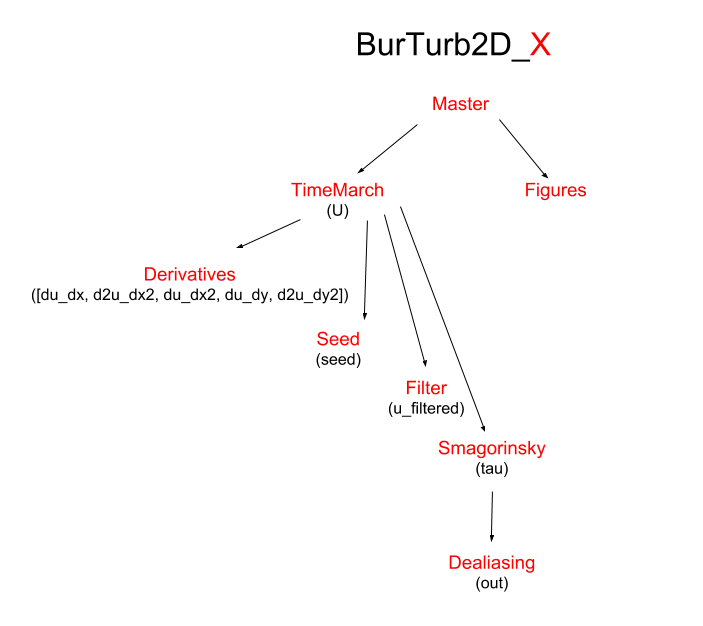
\includegraphics[width=0.5\textwidth]{Flow.png}
\caption{BurTurb2D code flow.} \label{fig:flow}
\end{figure}

To tackle this problem of implementing the Burger's equation with Smagorinsky's turbulence model\footnote{To follow the Smagorinksy model, I am referencing \href{https://www.cfd-online.com/Wiki/Smagorinsky-Lilly_model}{https://www.cfd-online.com/Wiki/Smagorinsky-Lilly\_model}, and using a $C_{s}=0.16$.}, I've decided to do some fun trickery and make a 2-dimensional simulation. However if I am to make this a two dimensional model, then it may be neat to observe some asymmetry. Thus, I am choosing a different initial condition than specified for the original simulation of Burger's equation, where we utilized an initial condition with a sine-wave. Our simulation domain ($x \times y$) will be $0\times0$ to $2\pi \times 2\pi$, however in the $x$-direction IC will be $u_{x}(x,y;t=0)=1-\cos(x(i))$ for all $i$, and for the $y$-direction, $u_{y}(x,y;t=0)=1-\cos(2y(j))$ where $\forall j<n_{y}/2 + 1$, otherwise the solution is flipped, i.e. $u_{y}(x,y;t=0)=-\left(1-\cos(2y)\right)$.

In order to solve this equation, we've reformatted it to incorporate two dimensions, and then effectively apply it twice in the code. The equation we are now using is,

$$ \partial_{t}u_{i} + u_{j}\partial_{j}u_{i} = -\frac{1}{2}\partial_{i}\tau_{ij} + \mathrm{seed},$$

\noindent where the diffusion term does not make way as we have set $\nu=0$. I have solved the 2D Burger's equation using a pseudo-spectral method. In my code I have broken up the components using functions in \texttt{MATLAB}, as illustrated in \ref{fig:flow}. Each component of the code will be delegated to it's own section in this document for easy finding. We have chosen to populate our space with 100 $n_{x}$ and $n_{y}$. Our time step is $0.51\times10^{3}$, as we found this to be the sweet spot before the solution goes unstable, and experiences a lot of numerical instability. Overall we hope to see two shocks colliding, or just about to collide.   

\newpage

\section{Master} \label{sec:master}

We utilize a \textbf{master}, or ``main,'' as referred to in Python nomenclature, where all the the effort done by the sub-function scripts refer back, and then provide results for the figures via the \textbf{master}. Here we initialize and the velocities in each direction, and specific the user inputs. We then calculate the initial condition for all $n_{x}$ and $n_{y}$. From there we calculate the initial superposition, or square-root of the two. Then we set things in motion utilizing the \textbf{Seed}, detailed in \ref{sec:seed}, via the \textbf{Time March} (\ref{sec:timemarch}). Using the \textbf{Time March}, we then calculate both \texttt{Ux} and \texttt{Uy}, then calculate the matrix \texttt{Z} so that we can plot the superposition of the two waves.

\vspace{50pt}

\begin{lstlisting}
%% Solves 2D Burgers Equation using Pseudo-spectral Method
% ~Marissa B. Adams~
%----------------------------------------------------------------------------
tic;
clc;
clear;
close all;

%% User-defined Inputs
n_x        = 100;           %ROWS
dx         = 2*pi/n_x;
n_y        = 100;           %COLUMNS
dy         = 2*pi/n_y;
t_steps    = 0.51e3;
dt         = 1e-3;
viscosity  = 0;                    %CHANGE IFF NEEDED

%% Calculations
% Initialize
% NOTES :: Starts from sinusoidal u,then take derivatives, introduce seed ...
% ... then introduce smag tau, use derivatives again to calculate the     ...
% ... derivative of tau, then calculate the RHS, then finite different to update

ux = zeros(n_x,1);
Ux = zeros(n_x,t_steps);
uy = zeros(n_y,1);
Uy = zeros(n_y,t_steps);

t = (0:dt:(t_steps-1)*dt)';
x = (0:dx:(n_x-1)*dx)';
y = (0:dy:(n_y-1)*dy)';

%%
for i=1:n_x
    for j=1:n_y
        ux(i,j,1)=1-cos(x(i));%sin(x(i));
        if(j<n_y/2+1)
            uy(i,j,1)=1-cos(2*(y(j)));%sin(y(j));
        else
            uy(i,j,1)=-(1-cos(2*y(j)));
        end
        Z(i,j,1) = sqrt(ux(i,j,1)^2 + uy(i,j,1)^2);
    end
end

%%
% Time-marching along x
seed_diff_x = 1e-6;                %CHANGE IFF NEEDED
seed_diff_y = 1e-6;
Ux = BurTurb2D_TimeMarch(ux,uy,viscosity,t_steps,dx,dy,dt,n_x,n_y,seed_diff_x);
ux = ux';
uy = uy';
Uy = BurTurb2D_TimeMarch(uy,ux,viscosity,t_steps,dy,dx,dt,n_y,n_x,seed_diff_y);

%% Plot figures
Z = zeros(n_x,n_y,t_steps);
for k = 1:t_steps
    for i=1:n_x
        for j=1:n_y
            Z(i,j,k) = sqrt(Ux(i,j,k)^2 + (Uy(j,i,k)')^2);
        end
    end
end


BurTurb2D_Figures(Z,Ux,Uy,ux,uy,x,y,t,dt,t_steps,n_x,n_y,viscosity);


%%
clearvars -except t x y Ux Uy Z viscosity n_x n_y dt dx dy t_steps
toc;
\end{lstlisting}

\newpage

\subsection{Time March} \label{sec:timemarch}

The \textbf{Time March} is effectively where all of the hard work goes into motion. For each time step, the derivatives and model are calculated for each side of the equation, and then updated.

\vspace{50pt}

\begin{lstlisting}
function U = BurTurb2D_TimeMarch(u,v,viscosity,t_steps,dx,dy,dt,n_x,n_y,seed_diff_x)
 for i = 1:t_steps
    [du_dx,d2u_dx2,du_dx2,du_dy,d2u_dy2] = BurTurb2D_Derivatives(u,dx,v,dy);
    seed_x                               = BurTurb2D_Seed(0.75,n_x,n_y)';
    seed_filtered_x                      = BurTurb2D_Filter(seed_x,2);  
    tau_x                                = BurTurb2D_Smagorinsky(u,du_dx,dx);
    dtau_xdx                             = BurTurb2D_Derivatives(tau_x,dx,tau_x,dy);
    
    RHS_x = viscosity*d2u_dx2 + viscosity*d2u_dy2 - 0.5*du_dx2 - v.*du_dy + ...
        sqrt(2*seed_diff_x/dt)*seed_filtered_x - 0.5*dtau_xdx;
    % FD for time dervative (velocity verlet-ish)
    if i == 1
        u_mod = u + dt*RHS_x;                              
    else
        u_mod = u + dt*(1.5*RHS_x - 0.5*RHS_xp);             
    end
    u_mod_k          = fft(u_mod);
    u_mod_k(n_x/2+1) = 0;
    u_mod            = real(ifft(u_mod_k));
    u                = u_mod;
    U(:,:,i)         = u_mod;
    RHS_xp           = RHS_x;
     
    fprintf('%f\n',i*dt);
    
 end
\end{lstlisting}

\newpage

\subsubsection{Derivatives} \label{sec:derivatives}

Here I've calculated the derivatives for the equation. Pretty self explanatory.

\vspace{50pt}

\begin{lstlisting}
%From notes
function [du_dx,d2u_dx2,du_dx2,du_dy,d2u_dy2] = BurTurb2D_Derivatives(u,dx,v,dy)

[n_x,n_y]    = size(u);

pre_x        = 2*pi/n_x/dx;
pre_y        = 2*pi/n_y/dy;

k_x          = [0 1:(n_x/2-1) 0 -(n_x/2-1):1:-1]';
k_y          = [0 1:(n_y/2-1) 0 -(n_y/2-1):1:-1]';

u_k          = fft2(u);
du_dx        = (pre_x)*real(ifft2(sqrt(-1)*k_x.*u_k));
d2u_dx2      = (pre_x^2)*real(ifft2(-k_x.*k_x.*u_k));

u_k_buffer   = [u_k(1:n_x/2+1,:)' zeros(n_y,n_x) u_k(n_x/2+2:n_x,:)']';
u_buffer     = real(ifft2(u_k_buffer));
u2_buffer    = u_buffer.*u_buffer;
u_k2_buffer  = fft2(u2_buffer);
u_k2         = [u_k2_buffer(1:n_x/2+1,:)' u_k2_buffer(n_x+n_x/2+2:n_x+n_x,:)']';
du_dx2       = (2)*(pre_x)*real(ifft2(sqrt(-1)*k_x.*u_k2));

v_k          = fft2(v);
du_dy        = (pre_y)*real(ifft2(sqrt(-1)*k_y.*v_k));
d2u_dy2      = (pre_y^2)*real(ifft2(-k_y.*k_y.*v_k));

end
\end{lstlisting}

\newpage

\subsubsection{Filter} \label{sec:filter}

Here I've apply a Large Eddy Simulation (LES) filter as described by the CFD-online wikipedia. One has the option of choosing a box or Gaussian filter. You can switch between the two in \textbf{Time March}. For this run, I used the Gaussian filter.  

\vspace{50pt}

\begin{lstlisting}
%Choose the box or gaussian, 1 or 2 respectively
%Formulas from CFD wiki: https://www.cfd-online.com/Wiki/LES_filters
function u_filtered = BurTurb2D_Filter(u,option)

n_x        = length(u);
delta      = (2*pi)/n_x;
u_k        = fft(u);
k          = [0 1:(n_x/2-1) n_x/2 -(n_x/2-1):1:-1]';

if option == 1      % Box Filter
    F               = sin(0.5*k*delta)./(0.5*k*delta);
    F(1)            = 1;
    u_proxy         = F.*u_k;
    u_proxy(n_x/2+1)= 0;
    
elseif option == 2  % Gaussian Filter
    F               = exp(-k.^2.*delta^2/24);
    F(1)            = 1;
    u_proxy         = F.*u_k;
    u_proxy(n_x/2+1)= 0;
end
u_filtered = real(ifft(u_proxy));

end
\end{lstlisting}

\newpage

\subsubsection{Seed} \label{sec:seed}

\begin{lstlisting}
%Copied from stack exchange
function seed = BurTurb2D_Seed(alpha,n_x,n_y)

lol                 = sqrt(n_x)*randn(n_x,n_y);
freq                = [ 1 1:n_x/2 (n_x/2-1):-1:1 ];
lol_k               = fft2(lol);
lol_k(1,:)            = 0; 
lol_k(n_x/2+1,:)      = 0;  
lol_mod             = lol_k .* (freq .^ (- alpha/2 ) );
seed                = real( ifft2(lol_mod) );

end
\end{lstlisting}

\vspace{-30pt}

\subsubsection{Smagorinsky} \label{sec:smagorinsky}

\begin{lstlisting}
function tau = BurTurb2D_Smagorinsky(u,du_dx,dx)

[n_x,n_y]      = size(u);
C_s_2          = 0.16^2; %from notes
mod_du_dx_smag = BurTurb2D_Dealiasing(abs(du_dx),n_x,n_y,1);
du_dx_smag     = BurTurb2D_Dealiasing(du_dx,n_x,n_y,1);
prod_du_dx     = BurTurb2D_Dealiasing(mod_du_dx_smag.*du_dx_smag,n_x,n_y,2);
tau            = -2*C_s_2*((dx)^2)*prod_du_dx;

end
\end{lstlisting}

\vspace{-30pt}

\paragraph{Dealiasing} \label{sec:dealiasing} \hspace{10pt}

\begin{lstlisting}
function out = BurTurb2D_Dealiasing(term,points1,points2,option)

if option == 1
    num1      = points1/2;
    out_k     = fft2(term);
    out_k_mod = [out_k(1:points1/2+1,:)' zeros(points2,num1) out_k(points1/2+2:points1,:)']';
    out       = real(ifft2(out_k_mod));
elseif option == 2
    num1                     = points1/2;
    out_k                    = fft2(term);
    out_k_mod                = [out_k(1:points1/2+1,:)' out_k(num1+points1/2+2:num1+points1,:)']';
    out_k_mod(points1/2+1,:) = 0;
    out                      = (3/2)*real(ifft2(out_k_mod));
    
end
\end{lstlisting}

\newpage

\subsection{Figures} \label{sec:figures}

\begin{lstlisting}
function BurTurb2D_Figures(Z,Ux,Uy,ux,uy,x,y,t,dt,t_steps,n_x,n_y, viscosity)
%%
[X,Y] = meshgrid(x(1:n_x),y(1:n_y));

CRed=zeros(100,100,3);
CRed(:,:,1)=1;

CGreen=zeros(100,100,3);
CGreen(:,:,2)=1;

CBlue=zeros(100,100,3);
CBlue(:,:,3)=1;

figure(1)
subplot(1,3,1)
surf(x,y,ux,CBlue,'FaceAlpha',0.5)%,'EdgeColor','none');
subplot(1,3,2)
surf(x,y,uy,CBlue,'FaceAlpha',0.5)%,'EdgeColor','none');
subplot(1,3,3)
surf(x,y,Z(:,:,1),CBlue,'FaceAlpha',0.5)%,'EdgeColor','none');
print('IC','-dpng');

figure(2)
surf(x,y,Ux(:,:,1),CBlue,'FaceAlpha',0.5)%,'EdgeColor','none')
hold on;
surf(x,y,Ux(:,:,end/2),CGreen,'FaceAlpha',0.5)%,'EdgeColor','none')
hold on;
surf(x,y,Ux(:,:,end),CRed,'FaceAlpha',0.5)%,'EdgeColor','none')
hold off;
print('UxTimeEvol','-dpng');

figure(3)
surf(x,y,Uy(:,:,1)',CBlue,'FaceAlpha',0.5)%,'EdgeColor','none')
hold on;
surf(x,y,Uy(:,:,end/2)',CGreen,'FaceAlpha',0.5)%,'EdgeColor','none')
hold on;
surf(x,y,Uy(:,:,end)',CRed,'FaceAlpha',0.5)%,'EdgeColor','none')
hold off;
print('UyTimeEvol','-dpng');

figure(5)
subplot(1,3,1)
%figure(5)
surf(X,Y,Z(1:n_x,1:n_y,1),CBlue,'FaceAlpha',0.5)%,'EdgeColor','none');
xlabel('x');
ylabel('y');
title(['t = ', num2str(t(1))]);

subplot(1,3,2)
%figure(6)
surf(X,Y,Z(1:n_x,1:n_y,t_steps/2),CGreen,'FaceAlpha',0.5)%,'EdgeColor','none');
xlabel('x');
ylabel('y');
title(['t = ', num2str(t(end)/2)]);

subplot(1,3,3)
%figure(7)
surf(X,Y,Z(1:n_x,1:n_y,t_steps-1),CRed,'FaceAlpha',0.5)%,'EdgeColor','none');
xlabel('x');
ylabel('y');
title(['t = ', num2str(t(end))]);
print('SuperPosVelEvolution','-dpng');

end
\end{lstlisting}

\newpage

\subsubsection{Results} \label{sec:results}

\begin{figure}[h]
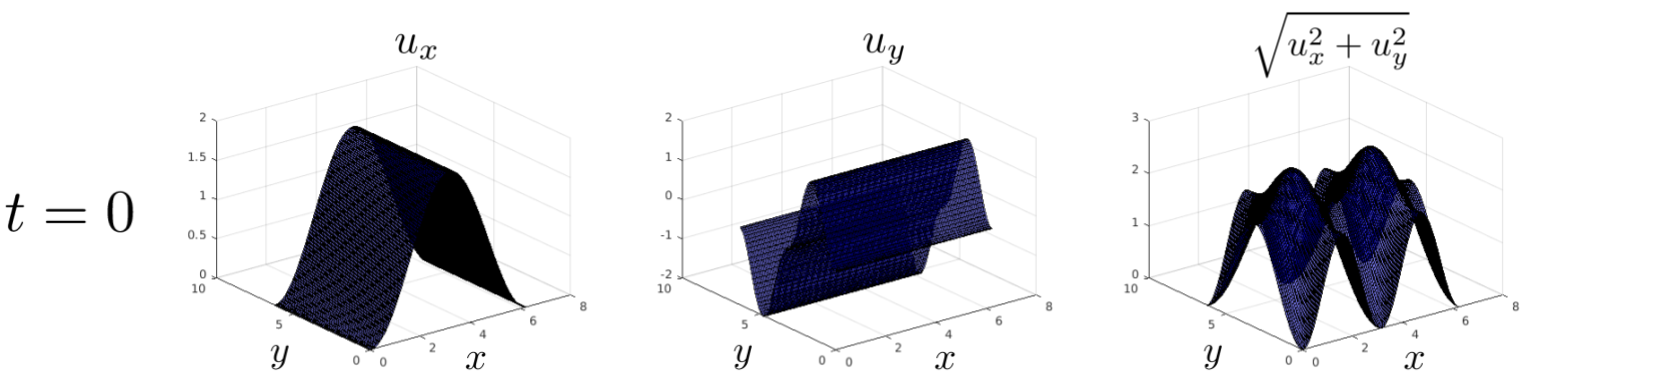
\includegraphics[width=\textwidth]{IC.png}
\end{figure}

\begin{tabular}{ c c }
\centering
  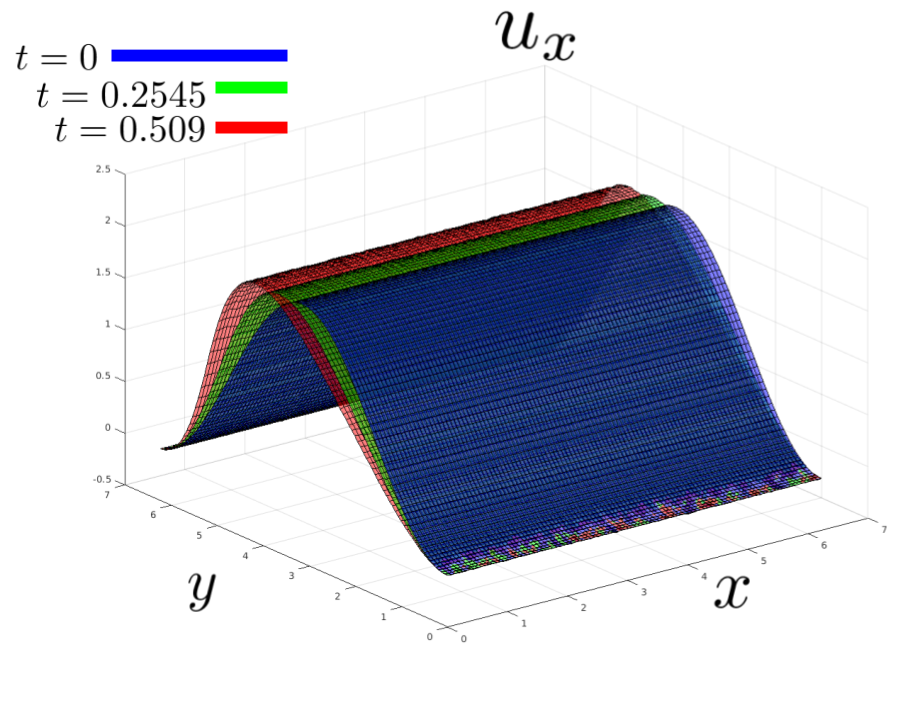
\includegraphics[width=0.45\textwidth]{UxTimeEvol.png} & 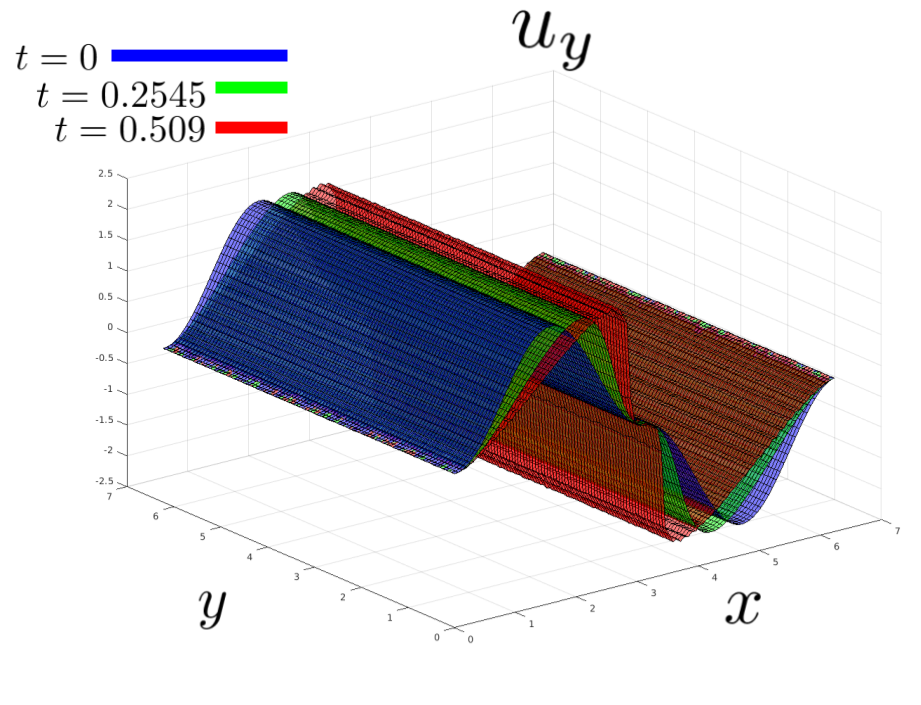
\includegraphics[width=0.45\textwidth]{UyTimeEvol.png} \\
\end{tabular}

\begin{figure}[h]
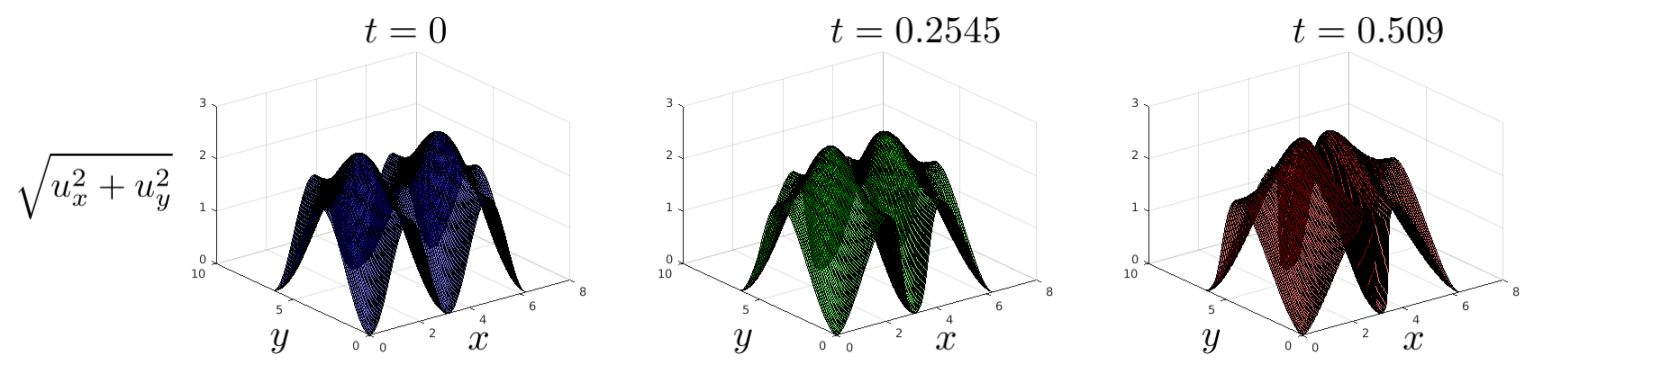
\includegraphics[width=\textwidth]{SuperPosVelEvolution.png}
\end{figure}

\textbf{Notes:}

Viewing the figures about as a table: 
\begin{itemize}
	\item \texttt{(row 1)} is the initial condition, from left to right we have the initial condition for $u_{x}$, $u_{y}$, and their mod-square combination, $U = \sqrt{u_{x}^{2} + u_{y}^{2}}$.
	\item \texttt{(row 2)} is the time evolution for both $u_{x}$ and $u_{y}$ for $t\approx\{0.0, 0.25, 0.5\}$. Continuing with \texttt{(row 1)}, you can see that the initial times are blue, the intermediate, green, and the final, red.
	\item \texttt{(row 3)} is the time evolution for the mod-square of the contents in \texttt{(row 2)}, following the same color pattern.
\end{itemize}

\end{document}